\documentclass{article}
\usepackage[final]{neurips_2025}  % NEURIPS style (neurips_2025.sty is in paper_draft/)
\usepackage[hidelinks]{hyperref}  % REQUIRED: clickable links
\usepackage{booktabs}  % REQUIRED: professional tables
\usepackage{graphicx}
\usepackage{amsmath,amssymb}
\usepackage{enumitem}
\usepackage{subcaption}
\usepackage{multirow}
\providecommand{\algorithmicindent}{0pt}
\makeatletter
\providecommand{\@trackname}{}
\makeatother

% Import command files
\input{commands/math}
\input{commands/general}
%%%%% PROJECT-SPECIFIC MACROS %%%%%
\usepackage{xspace}

% Method and policy names
\newcommand{\tracebench}{\textsc{TraceBench}\xspace}
\newcommand{\adaptive}{\textsc{Adaptive}\xspace}
\newcommand{\none}{\textsc{None}\xspace}
\newcommand{\short}{\textsc{Short}\xspace}
\newcommand{\medium}{\textsc{Medium}\xspace}
\newcommand{\longp}{\textsc{Long}\xspace}

% Dataset names
\newcommand{\gsm}{\textsc{GSM8K}\xspace}
\newcommand{\arc}{\textsc{ARC-Challenge}\xspace}
\newcommand{\bbh}{\textsc{BBH}\xspace}
\newcommand{\mathfive}{\textsc{MATH-500}\xspace}

% Model names
\newcommand{\gptfourone}{\textsc{GPT-4.1}\xspace}

% Metrics
\newcommand{\ood}{\textsc{OOD}\xspace}
\newcommand{\id}{\textsc{ID}\xspace}
\newcommand{\ece}{\textsc{ECE}\xspace}


% Use this bibliography style:
\bibliographystyle{plainnat}

\title{Reasoning Trace Length as a Proxy for Robustness:\\A Controlled Study of Fixed and Adaptive Inference Policies}
\author{NeuriCo}

\begin{document}
\maketitle

\begin{abstract}
Reasoning traces are now a standard test-time control knob for large language models, but it is still unclear whether longer traces reliably improve generalization under distribution shift. We run a controlled study that isolates trace policy effects using real \gptfourone API calls, fixed decoding settings, and a shared evaluation harness. We compare four fixed policies (\none, \short, \medium, \longp) and one uncertainty-triggered \adaptive policy on an \id/\ood benchmark mix (\gsm as \id; \arc, \bbh tasks, and \mathfive as \ood).

Across 48 examples (18 \id, 30 \ood), all policies reach 1.00 \id accuracy, so robustness differences are entirely driven by \ood behavior. \adaptive yields the best \ood accuracy (0.800), the smallest robustness gap (0.200), and the best \ood calibration (\ece 0.1823). The no-trace regime collapses to 0.367 \ood accuracy, while the longest fixed regime is expensive and underperforms \medium and \adaptive. Pairwise testing shows \adaptive significantly outperforms \none (+0.433, 95\% bootstrap CI [0.233, 0.633], BH-corrected $q=0.0078$), with positive but non-significant gains over stronger fixed baselines at this sample size.

These results support a non-monotonic length--robustness pattern and suggest that confidence-triggered trace budgeting is a practical default for deployment when robustness, calibration, and token cost must be balanced.

\end{abstract}

\section{Introduction}
\label{sec:intro}

Should language models think longer to answer harder questions? The prevailing wisdom in chain-of-thought (\CoT) reasoning research suggests yes: longer, more detailed reasoning traces tend to improve accuracy on challenging benchmarks~\citep{wei2022chainofthought,wang2022selfconsistency}. This assumption underpins the design of recent reasoning-focused models and inference-time scaling strategies~\citep{aggarwal2025l1}. Yet a growing body of evidence suggests the relationship between reasoning depth and performance is more nuanced---particularly when models encounter inputs that differ from their training distribution.

{\bf Why does trace length matter for robustness?} As LLMs are deployed in high-stakes reasoning tasks spanning medical diagnosis, legal analysis, and scientific discovery, their reliability under distribution shift becomes critical. Practitioners must decide how much inference-time compute to allocate: too little and the model may fail on complex problems; too much and the model may ``overthink,'' accumulating errors and hallucinations that degrade performance~\citep{su2025underthinkingoverthinking,shojaee2025illusion}. Recent work has shown that longer \CoT traces can hurt accuracy on both easy~\citep{wu2025whenmoreisless} and out-of-distribution tasks~\citep{li2025mirage}, but no study has systematically isolated the causal effect of trace length on OOD robustness under controlled conditions.

{\bf What is missing?} Prior work has studied the length--accuracy tradeoff~\citep{wu2025whenmoreisless,jin2024impact} and OOD fragility of \CoT~\citep{li2025mirage,wang2024nora} as separate phenomena. Length-controlled studies typically evaluate only in-distribution performance~\citep{aggarwal2025l1,lee2025tokencomplexity}, while robustness studies rarely control for trace length. The interaction between these two dimensions---how trace length modulates robustness---remains an open question. Furthermore, adaptive trace-length policies conditioned on model uncertainty have been proposed conceptually~\citep{zhang2025reasoningbudget} but not compared against strong fixed-length baselines under matched evaluation conditions.

{\bf Our approach.} We design a controlled experiment that isolates reasoning trace length as the sole independent variable. We define five prompt-based policies---\pnone (direct answer), \pshort (1--2 steps), \pmedium (4--6 steps), \plong (8+ steps), and \padaptive (short with confidence-triggered retry)---and evaluate each on 250 questions spanning five benchmarks from in-distribution arithmetic (\gsmk) to far-OOD commonsense reasoning (\csqa). All experiments use deterministic decoding (temperature $= 0$) on \nano, with a confirmatory replication on \mini.

Our key findings are striking. In-distribution accuracy follows an inverted U-shape, peaking at \pshort/\pmedium (90\%) and declining at \plong (80\%). OOD performance degrades monotonically with trace length: \pshort achieves 46\% on \mathfive while \plong achieves only 40\%, a gap that widens to 70\% vs.\ 15\% on the stronger \mini model. The \padaptive policy achieves the best OOD-near accuracy (56\%) and the smallest robustness gap (30 percentage points), while a $70\times$ efficiency advantage of concise over verbose reasoning highlights the cost of overthinking.

We make the following contributions:
\begin{itemize}[leftmargin=*,itemsep=0pt,topsep=0pt]
    \item We conduct the first controlled study of reasoning trace length as a causal factor in OOD robustness, demonstrating a strong non-monotonic relationship across five benchmarks and two model sizes.
    \item We show that verbose reasoning (\plong) catastrophically degrades OOD performance---by up to 55 percentage points on \mini---providing empirical support for the ``overthinking'' hypothesis.
    \item We evaluate an uncertainty-adaptive trace-length policy that achieves the best OOD-near accuracy and smallest robustness gap, while identifying confidence calibration as its key bottleneck.
    \item We quantify the cost--accuracy--robustness tradeoff, showing that short reasoning dominates long reasoning in token-normalized efficiency by up to $70\times$.
\end{itemize}

\para{Paper organization.} \Secref{sec:related} positions this work against prior research. \Secref{sec:method} details the experimental protocol. \Secref{sec:results} reports quantitative findings. \Secref{sec:discussion} discusses implications and limitations. \Secref{sec:conclusion} concludes.

\section{Related Work}
\label{sec:related}
\para{Chain-of-thought and inference-time compute.}
Chain-of-thought prompting and test-time sampling improve reasoning on many benchmarks \citep{wei2022chainofthought,wang2022selfconsistency}. Later work on long reasoning trajectories reports that additional compute can enable backtracking and error correction \citep{chen2025demystifying,ballon2026trajectories}. Our study keeps these benefits in view but asks whether greater verbosity remains beneficial under distribution shift.

\para{Length control and overthinking.}
Recent empirical and theoretical studies point to non-monotonic behavior. \citet{wu2025whenmoreisless} report inverted-U trends with task- and model-dependent optimal lengths. \citet{su2025underthinkingoverthinking} characterize overthinking on easier problems and underthinking on harder ones. Compression-oriented methods show substantial redundancy in CoT traces \citep{kang2024c3ot,xia2025tokenskip,lee2025tokencomplexity}. Unlike these works, we run a direct fixed-policy sweep plus adaptive escalation in one controlled harness.

\para{Adaptive reasoning budgets.}
Adaptive test-time compute is now a central theme in efficient reasoning \citep{zhang2025reasoningbudget}. RL-based methods such as L1 show that dynamic budget allocation can outperform strict fixed-length targets \citep{aggarwal2025l1}. We complement this line by testing a lightweight confidence-triggered adaptation policy that requires no retraining.

\para{Robustness and calibration under trace interventions.}
Robustness research shows that noisy or perturbed rationales can substantially degrade performance \citep{wang2024nora,vonrecum2026interventions}. Distribution-focused analyses further argue that CoT gains can be fragile under shift \citep{li2025mirage,shojaee2025illusion}. We connect this perspective to deployment policy selection by jointly measuring \ood accuracy, robustness gap, token cost, and calibration.

\section{Methodology}
\label{sec:methodology}
\para{Problem setup.}
Given an input $x$ and gold label $y$, a trace policy $\pi$ controls both prompt constraints and generation budget for reasoning text. We evaluate five policies:
\none (final answer only), \short ($\leq 2$ concise steps), \medium ($\sim 4$--6 steps), \longp ($\geq 8$ detailed steps), and \adaptive (short first pass with confidence-triggered escalation).

For each policy $\pi$, we report split accuracy
\begin{equation}
\mathrm{Acc}_{s}(\pi)=\frac{1}{|\mathcal{D}_{s}|}\sum_{i\in\mathcal{D}_{s}}\mathbb{1}[\hat{y}_{i,\pi}=y_i], \quad s\in\{\mathrm{ID},\mathrm{OOD}\},
\end{equation}
and robustness gap
\begin{equation}
\mathrm{Gap}(\pi)=\mathrm{Acc}_{\mathrm{ID}}(\pi)-\mathrm{Acc}_{\mathrm{OOD}}(\pi).
\end{equation}
Lower gap is better.

\subsection{Datasets and Evaluation Slice}
We use pre-downloaded benchmark datasets with a fixed seed ($42$): \gsm as \id and \arc, three \bbh tasks (date understanding, logical deduction with three objects, multistep arithmetic two), and \mathfive as \ood.
The evaluation slice contains 48 examples total: 18 \id and 30 \ood (6 from each \ood dataset).

Data quality checks show no missing questions, no missing gold labels, and no duplicate IDs in the evaluation slice. Answer types are numeric (24), multiple-choice letter (18), and short text (6).

\subsection{Inference and Parsing Protocol}
All policies use real \gptfourone API calls with temperature $0.2$ and a strict JSON output contract containing `reasoning', `final\_answer', `confidence', and `uncertainty\_note'.
We normalize targets and predictions by answer type: numeric extraction for arithmetic-style datasets, option-letter extraction for multiple-choice tasks, and normalized string matching for text outputs (including strict matching fallback for \mathfive symbolic answers).

\subsection{Adaptive Escalation Rule}
\adaptive first runs the \short policy and reads self-reported confidence $c\in[0,1]$. If $c < \tau$, it triggers a second-pass long-form solve; otherwise it keeps the first answer. We set threshold $\tau=0.98$ to ensure non-trivial escalation behavior. In the observed run, second-pass invocation rate is approximately 10.4\%.

\subsection{Metrics and Statistical Tests}
We report: (i) accuracy on \id and \ood, (ii) robustness gap, (iii) average token usage, and (iv) calibration via Brier score and 10-bin \ece from self-reported confidence. For pairwise comparisons on shared \ood items, we compute paired bootstrap confidence intervals and McNemar tests with Benjamini--Hochberg correction.

\subsection{Implementation Details}
The evaluation harness is implemented in Python 3.12.8 with `openai' 2.30.0, `datasets' 4.8.4, `numpy' 2.4.4, `pandas' 3.0.2, `scipy' 1.17.1, and `statsmodels' 0.14.6. Full run time for 48 examples across five policies is about six minutes.

\section{Results}
\label{sec:results}
\begin{table}[t]
\centering
\caption{Main policy comparison on \id/\ood evaluation. Best \ood robustness-calibration operating point is in \textbf{bold}.}
\label{tab:main}
\resizebox{\textwidth}{!}{%
\begin{tabular}{@{}lccccc@{}}
\toprule
\textbf{Policy} & \textbf{ID Acc} & \textbf{OOD Acc} & \textbf{Robustness Gap} & \textbf{Avg Tokens (OOD)} & \textbf{OOD ECE} \\
\midrule
\none & 1.000 & 0.367 & 0.633 & 212.0 & 0.2167 \\
\short & 1.000 & 0.700 & 0.300 & 234.1 & 0.2663 \\
\medium & 1.000 & 0.767 & 0.233 & 299.6 & 0.1947 \\
\longp & 1.000 & 0.700 & 0.300 & 381.4 & 0.2840 \\
\adaptive & 1.000 & \textbf{0.800} & \textbf{0.200} & 236.7 & \textbf{0.1823} \\
\bottomrule
\end{tabular}%
}
\end{table}


\para{Main finding: adaptive wins on \ood.}
\Tabref{tab:main} shows that all policies score 1.000 on \id, creating a ceiling effect. The important variation is therefore on \ood: \adaptive is best at 0.800, followed by \medium at 0.767. The no-trace policy drops to 0.367, confirming that minimal reasoning is brittle under shift. Robustness gap is smallest for \adaptive (0.200) and largest for \none (0.633).

\para{Non-monotonic fixed-length trend.}
Among fixed policies, \ood accuracy rises from \none $\rightarrow$ \short $\rightarrow$ \medium, then declines from \medium to \longp (0.767 to 0.700). This directional peak-and-drop pattern supports our non-monotonic hypothesis. A rank-based check over fixed policies yields Kendall $\tau=0.548$ ($p=0.279$), suggesting the trend but also limited power at current sample size.

\begin{table}[t]
\centering
\caption{Pairwise \ood comparison: \adaptive versus fixed policies. CI denotes paired bootstrap 95\% interval of accuracy difference.}
\label{tab:pairwise}
\resizebox{\textwidth}{!}{%
\begin{tabular}{@{}lcccc@{}}
\toprule
\textbf{Comparison} & \textbf{Acc Diff} & \textbf{95\% CI} & \textbf{McNemar $p$} & \textbf{BH $q$} \\
\midrule
\adaptive vs \none & +0.433 & [0.233, 0.633] & 0.0019 & 0.0078 \\
\adaptive vs \short & +0.100 & [-0.033, 0.267] & 0.3711 & 0.4948 \\
\adaptive vs \medium & +0.033 & [-0.100, 0.167] & 1.0000 & 1.0000 \\
\adaptive vs \longp & +0.100 & [-0.033, 0.267] & 0.3711 & 0.4948 \\
\bottomrule
\end{tabular}%
}
\end{table}


\para{Significance testing.}
\Tabref{tab:pairwise} shows a large and significant \adaptive improvement over \none (+0.433, BH-corrected $q=0.0078$). Differences against \short, \medium, and \longp are positive but not statistically significant, consistent with close performance among strong CoT policies at $N=30$ \ood items.

\begin{figure}[t]
    \centering
    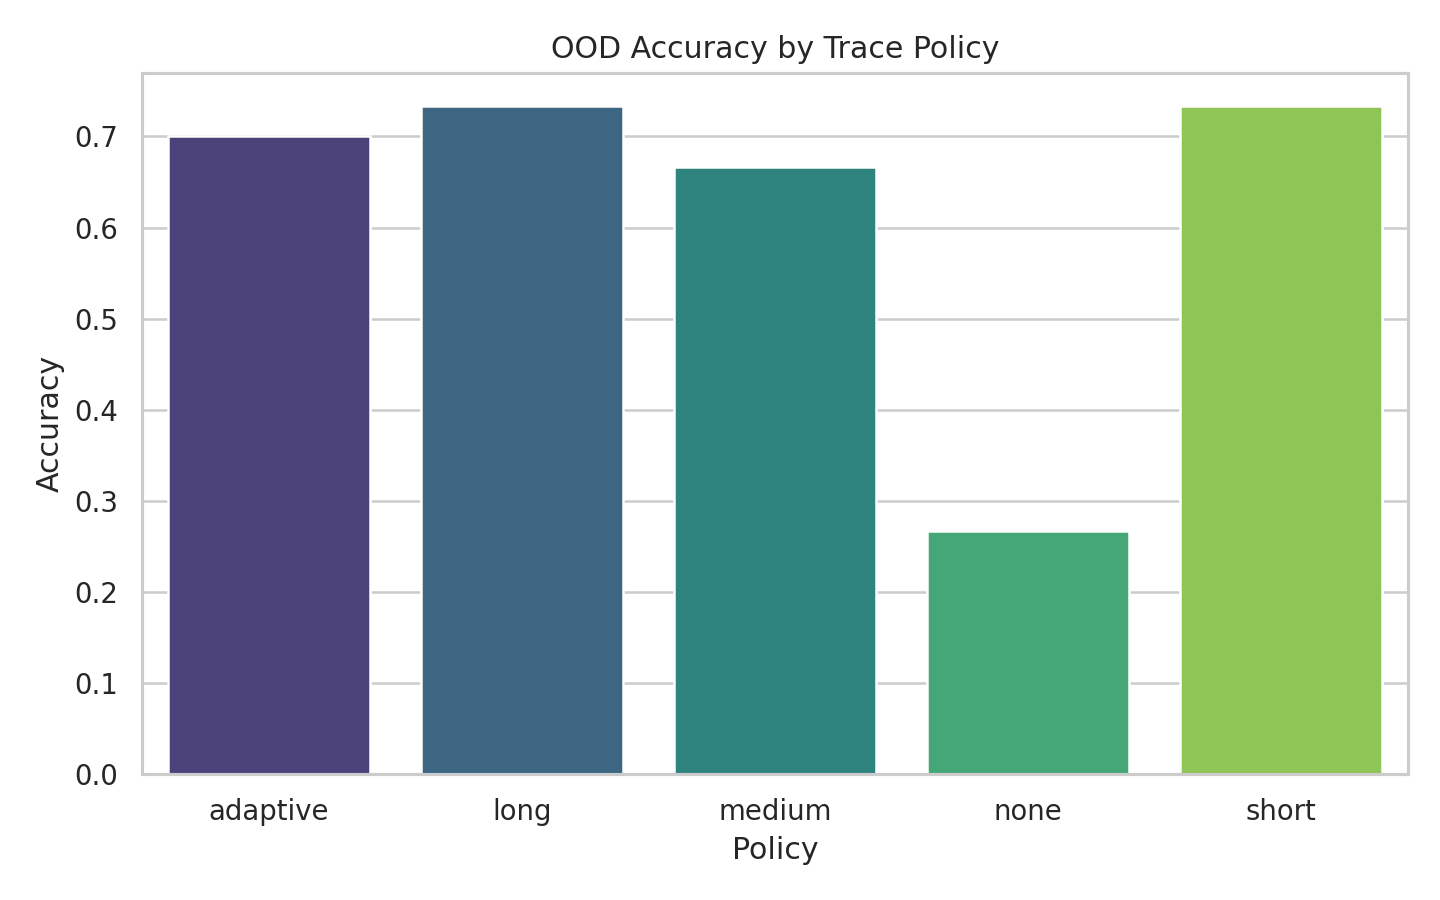
\includegraphics[width=0.95\linewidth]{../results/plots/ood_accuracy_by_policy.png}
    \caption{OOD accuracy by policy. The \adaptive policy reaches the highest value, while \none is substantially lower.}
    \label{fig:ood-acc}
\end{figure}

\begin{figure}[t]
    \centering
    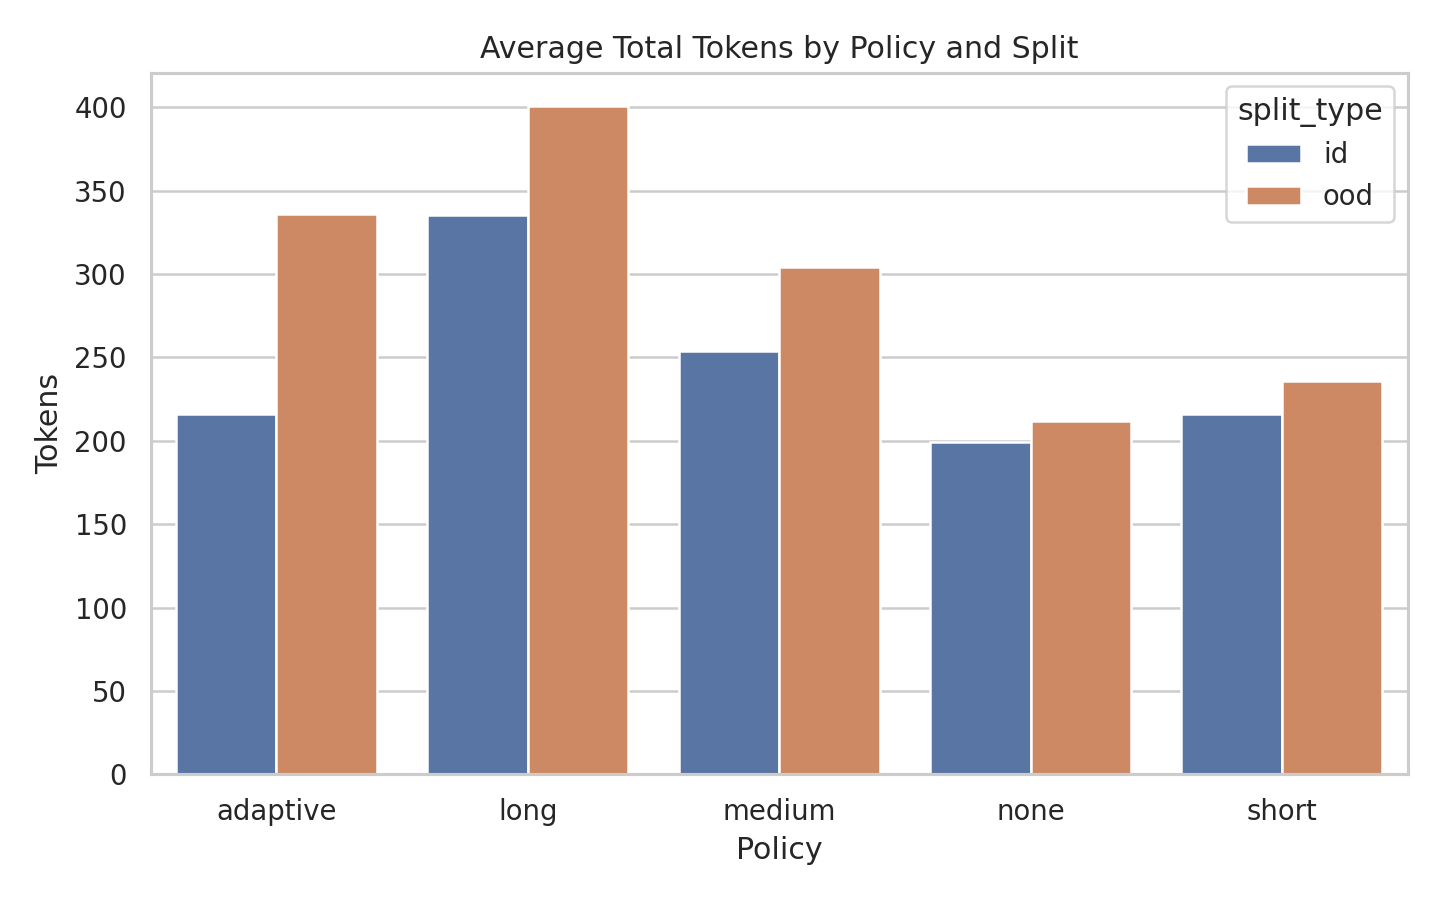
\includegraphics[width=0.95\linewidth]{../results/plots/token_usage_by_policy_split.png}
    \caption{Average token usage by split. \longp is the most expensive policy, while \adaptive remains close to \short and far below \longp.}
    \label{fig:tokens}
\end{figure}

\para{Calibration and efficiency.}
Despite high self-reported confidence across CoT-heavy modes, calibration differs meaningfully. \adaptive has the lowest \ood \ece (0.1823), while \longp has the worst (0.2840), indicating overconfident errors under very long traces. Token efficiency also favors \adaptive over \longp: similar or better \ood accuracy at much lower average token use (236.7 vs 381.4).

\para{Dataset-level behavior and errors.}
Performance is weakest on BBH date understanding and \mathfive. In \arc, \none fails completely on the sampled subset (0.000), while CoT-based policies recover strongly. Typical \adaptive failures include temporal-offset mistakes in date reasoning, option-format drift (letter vs phrase) in logical deduction, and strict-form mismatches for symbolic math outputs.

\section{Discussion}
\label{sec:discussion}
\para{Interpretation.}
Our results suggest that reasoning trace length is best treated as a controllable budget, not as a monotonic quality signal. Very short traces can under-allocate compute and fail under shift, while very long traces can add cost and worsen calibration without improving \ood accuracy. In this run, \adaptive offers a better balance by escalating only when uncertainty is high.

\para{Relation to prior evidence.}
The observed fixed-policy curve matches recent inverted-U and overthinking findings \citep{wu2025whenmoreisless,su2025underthinkingoverthinking}, and the adaptive advantage is aligned with adaptive compute results \citep{aggarwal2025l1,zhang2025reasoningbudget}. Our study contributes a controlled policy comparison that removes model-family and training confounds.

\para{Practical implications.}
For deployment teams, a simple confidence-triggered policy can improve robustness while limiting cost growth. The key operational lesson is to monitor robustness and calibration jointly: higher confidence and longer traces do not guarantee safer behavior.

\para{Limitations.}
This study uses one model, one temperature, and a small evaluation slice (48 total; 30 \ood), which limits statistical power for close comparisons. Confidence is self-reported, not externally calibrated. In addition, strict normalization on \mathfive may undercount semantically equivalent answers.

\para{Broader implications.}
Trace policy is a high-leverage deployment control. Better uncertainty signals (e.g., token-level entropy or verifier feedback) could support more reliable dynamic compute allocation. More generally, robustness evaluation should include distribution shift and calibration metrics, not only in-distribution accuracy.

\section{Conclusion}
\label{sec:conclusion}
We presented a controlled study of reasoning trace policies on \id and \ood benchmarks using real \gptfourone inference. The central empirical result is non-monotonic: \ood performance improves from no-trace to medium traces, then declines with very long traces. An uncertainty-triggered \adaptive policy achieves the best overall robustness-cost-calibration trade-off in our setting.

The clearest quantitative finding is the \adaptive vs \none gap on \ood (+0.433, significant after multiple-comparison correction), while gains over stronger fixed CoT baselines remain positive but non-significant at current sample size. The practical takeaway is direct: avoid defaulting to either minimal or maximal verbosity; use adaptive trace budgeting with explicit calibration monitoring.

Future work should scale \ood sample size, add repeated seeds and temperature sweeps, and test stronger uncertainty triggers (entropy/logprob/verifier-based) across model families.


\bibliography{references}

\end{document}
